% Options for packages loaded elsewhere
\PassOptionsToPackage{unicode}{hyperref}
\PassOptionsToPackage{hyphens}{url}
%
\documentclass[
  man]{apa6}
\usepackage{amsmath,amssymb}
\usepackage{iftex}
\ifPDFTeX
  \usepackage[T1]{fontenc}
  \usepackage[utf8]{inputenc}
  \usepackage{textcomp} % provide euro and other symbols
\else % if luatex or xetex
  \usepackage{unicode-math} % this also loads fontspec
  \defaultfontfeatures{Scale=MatchLowercase}
  \defaultfontfeatures[\rmfamily]{Ligatures=TeX,Scale=1}
\fi
\usepackage{lmodern}
\ifPDFTeX\else
  % xetex/luatex font selection
\fi
% Use upquote if available, for straight quotes in verbatim environments
\IfFileExists{upquote.sty}{\usepackage{upquote}}{}
\IfFileExists{microtype.sty}{% use microtype if available
  \usepackage[]{microtype}
  \UseMicrotypeSet[protrusion]{basicmath} % disable protrusion for tt fonts
}{}
\makeatletter
\@ifundefined{KOMAClassName}{% if non-KOMA class
  \IfFileExists{parskip.sty}{%
    \usepackage{parskip}
  }{% else
    \setlength{\parindent}{0pt}
    \setlength{\parskip}{6pt plus 2pt minus 1pt}}
}{% if KOMA class
  \KOMAoptions{parskip=half}}
\makeatother
\usepackage{xcolor}
\usepackage{graphicx}
\makeatletter
\def\maxwidth{\ifdim\Gin@nat@width>\linewidth\linewidth\else\Gin@nat@width\fi}
\def\maxheight{\ifdim\Gin@nat@height>\textheight\textheight\else\Gin@nat@height\fi}
\makeatother
% Scale images if necessary, so that they will not overflow the page
% margins by default, and it is still possible to overwrite the defaults
% using explicit options in \includegraphics[width, height, ...]{}
\setkeys{Gin}{width=\maxwidth,height=\maxheight,keepaspectratio}
% Set default figure placement to htbp
\makeatletter
\def\fps@figure{htbp}
\makeatother
\setlength{\emergencystretch}{3em} % prevent overfull lines
\providecommand{\tightlist}{%
  \setlength{\itemsep}{0pt}\setlength{\parskip}{0pt}}
\setcounter{secnumdepth}{-\maxdimen} % remove section numbering
% Make \paragraph and \subparagraph free-standing
\ifx\paragraph\undefined\else
  \let\oldparagraph\paragraph
  \renewcommand{\paragraph}[1]{\oldparagraph{#1}\mbox{}}
\fi
\ifx\subparagraph\undefined\else
  \let\oldsubparagraph\subparagraph
  \renewcommand{\subparagraph}[1]{\oldsubparagraph{#1}\mbox{}}
\fi
% definitions for citeproc citations
\NewDocumentCommand\citeproctext{}{}
\NewDocumentCommand\citeproc{mm}{%
  \begingroup\def\citeproctext{#2}\cite{#1}\endgroup}
\makeatletter
 % allow citations to break across lines
 \let\@cite@ofmt\@firstofone
 % avoid brackets around text for \cite:
 \def\@biblabel#1{}
 \def\@cite#1#2{{#1\if@tempswa , #2\fi}}
\makeatother
\newlength{\cslhangindent}
\setlength{\cslhangindent}{1.5em}
\newlength{\csllabelwidth}
\setlength{\csllabelwidth}{3em}
\newenvironment{CSLReferences}[2] % #1 hanging-indent, #2 entry-spacing
 {\begin{list}{}{%
  \setlength{\itemindent}{0pt}
  \setlength{\leftmargin}{0pt}
  \setlength{\parsep}{0pt}
  % turn on hanging indent if param 1 is 1
  \ifodd #1
   \setlength{\leftmargin}{\cslhangindent}
   \setlength{\itemindent}{-1\cslhangindent}
  \fi
  % set entry spacing
  \setlength{\itemsep}{#2\baselineskip}}}
 {\end{list}}
\usepackage{calc}
\newcommand{\CSLBlock}[1]{\hfill\break\parbox[t]{\linewidth}{\strut\ignorespaces#1\strut}}
\newcommand{\CSLLeftMargin}[1]{\parbox[t]{\csllabelwidth}{\strut#1\strut}}
\newcommand{\CSLRightInline}[1]{\parbox[t]{\linewidth - \csllabelwidth}{\strut#1\strut}}
\newcommand{\CSLIndent}[1]{\hspace{\cslhangindent}#1}
\ifLuaTeX
\usepackage[bidi=basic]{babel}
\else
\usepackage[bidi=default]{babel}
\fi
\babelprovide[main,import]{english}
% get rid of language-specific shorthands (see #6817):
\let\LanguageShortHands\languageshorthands
\def\languageshorthands#1{}
% Manuscript styling
\usepackage{upgreek}
\captionsetup{font=singlespacing,justification=justified}

% Table formatting
\usepackage{longtable}
\usepackage{lscape}
% \usepackage[counterclockwise]{rotating}   % Landscape page setup for large tables
\usepackage{multirow}		% Table styling
\usepackage{tabularx}		% Control Column width
\usepackage[flushleft]{threeparttable}	% Allows for three part tables with a specified notes section
\usepackage{threeparttablex}            % Lets threeparttable work with longtable

% Create new environments so endfloat can handle them
% \newenvironment{ltable}
%   {\begin{landscape}\centering\begin{threeparttable}}
%   {\end{threeparttable}\end{landscape}}
\newenvironment{lltable}{\begin{landscape}\centering\begin{ThreePartTable}}{\end{ThreePartTable}\end{landscape}}

% Enables adjusting longtable caption width to table width
% Solution found at http://golatex.de/longtable-mit-caption-so-breit-wie-die-tabelle-t15767.html
\makeatletter
\newcommand\LastLTentrywidth{1em}
\newlength\longtablewidth
\setlength{\longtablewidth}{1in}
\newcommand{\getlongtablewidth}{\begingroup \ifcsname LT@\roman{LT@tables}\endcsname \global\longtablewidth=0pt \renewcommand{\LT@entry}[2]{\global\advance\longtablewidth by ##2\relax\gdef\LastLTentrywidth{##2}}\@nameuse{LT@\roman{LT@tables}} \fi \endgroup}

% \setlength{\parindent}{0.5in}
% \setlength{\parskip}{0pt plus 0pt minus 0pt}

% Overwrite redefinition of paragraph and subparagraph by the default LaTeX template
% See https://github.com/crsh/papaja/issues/292
\makeatletter
\renewcommand{\paragraph}{\@startsection{paragraph}{4}{\parindent}%
  {0\baselineskip \@plus 0.2ex \@minus 0.2ex}%
  {-1em}%
  {\normalfont\normalsize\bfseries\itshape\typesectitle}}

\renewcommand{\subparagraph}[1]{\@startsection{subparagraph}{5}{1em}%
  {0\baselineskip \@plus 0.2ex \@minus 0.2ex}%
  {-\z@\relax}%
  {\normalfont\normalsize\itshape\hspace{\parindent}{#1}\textit{\addperi}}{\relax}}
\makeatother

% \usepackage{etoolbox}
\makeatletter
\patchcmd{\HyOrg@maketitle}
  {\section{\normalfont\normalsize\abstractname}}
  {\section*{\normalfont\normalsize\abstractname}}
  {}{\typeout{Failed to patch abstract.}}
\patchcmd{\HyOrg@maketitle}
  {\section{\protect\normalfont{\@title}}}
  {\section*{\protect\normalfont{\@title}}}
  {}{\typeout{Failed to patch title.}}
\makeatother

\usepackage{xpatch}
\makeatletter
\xapptocmd\appendix
  {\xapptocmd\section
    {\addcontentsline{toc}{section}{\appendixname\ifoneappendix\else~\theappendix\fi\\: #1}}
    {}{\InnerPatchFailed}%
  }
{}{\PatchFailed}
\keywords{Need for Cognition, burnout, self-control, emotion regulation, coping\newline\indent Word count: X}
\DeclareDelayedFloatFlavor{ThreePartTable}{table}
\DeclareDelayedFloatFlavor{lltable}{table}
\DeclareDelayedFloatFlavor*{longtable}{table}
\makeatletter
\renewcommand{\efloat@iwrite}[1]{\immediate\expandafter\protected@write\csname efloat@post#1\endcsname{}}
\makeatother
\usepackage{lineno}

\linenumbers
\usepackage{csquotes}
\ifLuaTeX
  \usepackage{selnolig}  % disable illegal ligatures
\fi
\usepackage{bookmark}
\IfFileExists{xurl.sty}{\usepackage{xurl}}{} % add URL line breaks if available
\urlstyle{same}
\hypersetup{
  pdftitle={Need for Cognition and Burnout in healthcare: The mediating role of self-control, emotion regulation, and coping strategies},
  pdfauthor={Kea Rüter1, Alexander Strobel2, \& Anja Strobel1},
  pdflang={en-EN},
  pdfkeywords={Need for Cognition, burnout, self-control, emotion regulation, coping},
  hidelinks,
  pdfcreator={LaTeX via pandoc}}

\title{Need for Cognition and Burnout in healthcare: The mediating role of self-control, emotion regulation, and coping strategies}
\author{Kea Rüter\textsuperscript{1}, Alexander Strobel\textsuperscript{2}, \& Anja Strobel\textsuperscript{1}}
\date{}


\shorttitle{NFC and Burnout in healthcare}

\authornote{

Alexander Strobel: \url{https://orcid.org/0000-0002-9426-5397}

Anja Strobel: \url{https://orcid.org/0000-0002-0313-0615}

The authors made the following contributions. Kea Rüter: Writing - Original Draft, Data Curation, Formal Analysis; Alexander Strobel: Conceptualization, Writing - Review \& Editing, Supervision; Anja Strobel: Conceptualization, Writing - Review \& Editing, Supervision.

Correspondence concerning this article should be addressed to Anja Strobel, Technische Universität Chemnitz, Department of Psychology, Wilhelm-Raabe-Straße 43, 09120 Chemnitz, Germany. E-mail: \href{mailto:anja.strobel@psychologie.tu-chemnitz.de}{\nolinkurl{anja.strobel@psychologie.tu-chemnitz.de}}

}

\affiliation{\vspace{0.5cm}\textsuperscript{1} Department of Psychology, Technische Universität Chemnitz, Chemnitz, Germany\\\textsuperscript{2} Faculty of Psychology, Technische Universität Dresden, Dresden, Germany}

\abstract{%
Burnout has emerged as a global health concern, with its prevalence notably increasing during the COVID-19 pandemic.
This especially occurs among individuals working within the field of healthcare.
In order to contribute to the improvement of working conditions and mental health, this study replicates a mediation model previously tested by Grass et al.~(2018) among teaching students and by Zerna, Engelmann et al.~(2022) among teachers.
For this purpose, multiple mediation models, using a sample of N = 642 healthcare workers were examined.
The incorporated predictor was Need for Cognition (an intrinsic motivation to engage with cognitively demanding thoughts).
Mediators were self-control, the emotion regulation strategies reappraisal and suppression, as well as adaptive and maladaptive coping strategies.
The burnout subdimensions reduced personal efficacy, emotional exhaustion, and depersonalization each functioned individually as outcome variables.
In addition to the mediation analyses, correlation analyses of these variables were also calculated.
The results confirmed that adaptive coping strategies functioned preventively across all burnout dimensions.
Furthermore, reappraisal and maladaptive coping mediated the relationship between NFC and some subdimensions of burnout.
Healthcare workers who tended towards higher NFC appeared to be protected from burnout development due to various tested mediators.
Regarding the daily work environment, initial evidence suggests that efforts should be made to particularly promote adaptive coping strategies.
Future studies should further examine the link between NFC and burnout among healthcare professionals.
}



\begin{document}
\maketitle

Burnout is a psychological, work-related stress syndrome and a global health concern (\textbf{parandeh\_prevalence\_2022?}).
It correlates with depression (Bianchi et al., 2015), increased alcohol abuse (Oreskovich, 2012), and a heightened risk of suicidal thoughts (Shanafelt et al., 2011).
As a response to excessive work stress (Maslach, 1998), burnout affects not only individuals but also their workplace (West et al., 2018), leading to decreased productivity (Dewa et al., 2017), reduced job satisfaction, and intentions to leave the profession (Shanafelt et al., 2009).

Occupational stress is a growing problem, especially among healthcare workers (Hassan et al., 2020).
Challenges like time constraints, lack of control, and competing demands are significant job strains (Lyndon, 2015).
The COVID-19 pandemic further exacerbated burnout rates (Galanis et al., 2021; Prasad et al., 2021), as healthcare workers faced higher health risks, increased workloads, inadequate equipment, and limited resources.
These strains impacted not only the workers but also the quality of patient care, leading to lower patient satisfaction and increased medical errors (West et al., 2018).

The rising number of burnout cases underscores its significance in today's society.
Despite extensive research, the exact causes and antecedents of burnout are not fully understood.
This study investigates the relationship between burnout, its underlying mechanisms, and protective factors, extending previous research on factors mediating the role of cognitive motivation in burnout (Grass et al., 2018; Zerna et al., 2022) from aspiring and experienced teachers to healthcare professionals.
The following section explains the mediation model and its variables.

\subsection{Theoretical Framework}\label{theoretical-framework}

\ldots{}

\section{Methods}\label{methods}

We report how we determined our sample size, all data exclusions, all manipulations, and all measures in the study (cf. Simmons et al., 2012).

\subsection{Study design}\label{study-design}

The preregistration of the current study is available at \url{https://osf.io/d6y9k}.
Data acquisition took place at two separate assessment occasions (Kadur, 2018; Ziessler, 2019).
Data were assessed via anonymous, cross-sectional online surveys using the Enterprise Feedback Suite Survey platform (EFS, Questback, 2017).
Participants were informed about the study's objectives, duration, and data security.
Further, they were given the opportunity to participate in a cash raffle, where €25 were handed out to two participants for every 100 individuals who took part in the study.
As additional reimbursement, participants were offered to receive the study results on request as well as information on the personal and work-related risk factors of burnout.
Before the subjects reported demographic information and completed the questionnaires, participants declared their consent for data security and study participation.
At the end of the survey, a control item was included to ensure that participants indicated whether they answered the questions sincerely.
Finally, those interested in the raffle could provide their email address which was recorded separately from the scientific data.

\subsection{Participants}\label{participants}

\ldots{}

\subsection{Material}\label{material}

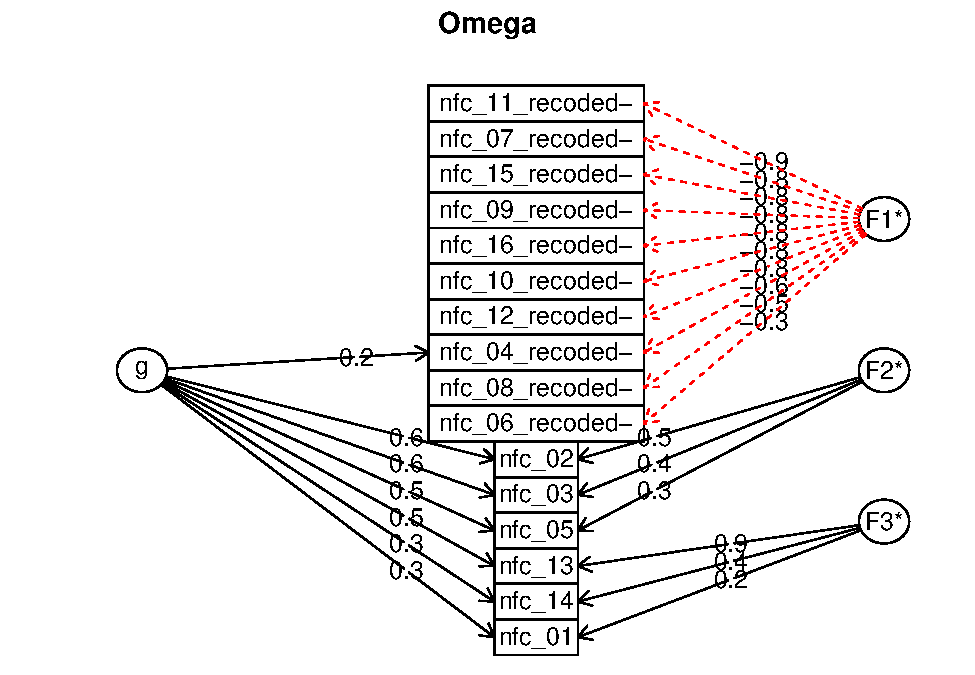
\includegraphics{NFC-Caregiver_files/figure-latex/omega-1.pdf}

All questionnaires used were administered in German language.
The reliabilities (MacDonald's \(\omega\) and Cronbach's \(\alpha\)) of the inventories used can be found in Table 1.
The burnout dimensions \emph{reduced personal efficiency}, \emph{emotional exhaustion}, and \emph{depersonalization} were assessed using the German version of the 22-item Maslach Burnout Inventory (MBI-D, Büssing \& Perrar, 1992).
Items such as ``I feel burned out by my job.'' were rated on a scale from 1 (does not occur at all) to 6 (occurs very often/strongly).
The internal consistencies of the MBI-D showed good to excellent reliabilities (MacDonald's \(\omega\) \textgreater{} .82).
For clearer classification of each subdimension's individual expressions, Dreher et al. (2019) provided specific values, where high burnout expression is classsified at rPE values \textgreater{} 24, EE values \textgreater{} 22, and DE values \textgreater{} 8.
NFC was assessed with the 16-item short version of the German NFC scale (NCS, Bless et al., 1994) with items like ``I like it when my life is full of tricky tasks that I have to solve.'' These items were rated on a seven-point rating scale ranging from +3 (very accurate) to --3 (completely inaccurate).
The scale demonstrated an excellent internal consistency of MacDonald's \(\omega\) \textgreater{} .91.
Self-control was measured by the 13-item short form of the Self-Control Scale (SCS-K-D, Bertrams \& Dickhäuser, 2009).
Here, a five-point Likert scale from 1 (completely inaccurate) to 5 (completely accurate) was used to answer questions like ``I am good at resisting temptations.''
This scale showed an acceptable internal consistency of MacDonald's \(\omega\) \textgreater{} .79.
Further, the Emotion Regulation Questionnaire (ERQ-D, Abler \& Kessler, 2009), which included 10 items, was used to assess reappraisal and suppression. Reappraisal was measured by items like ``When I get into a stressful situation, I change my thoughts about the situation, so it calms me down.''
Suppression was determined by items such as ``I keep my feelings to myself.''
Participants responded on a scale ranging from 1 (not true at all) to 7 (absolutely true).
The subscale that assessed reappraisal contained six items and achieved good reliability (MacDonald's \(\omega\) \textgreater{} .86).
The four-item suppression subscale of the ERQ-D also reached good reliability with MacDonald's \(\omega\) \textgreater{} .81.
Finally (and differing from the material used by Grass et al. (2018)), the 20-item Stress and Coping Inventory (SCI, Satow, 2012) was used to measure adaptive as well as maladaptive coping strategies.
Adaptive coping was assessed by the subscales ``positive thinking'', ``active stress management'', ``social support'', and ``holding on to faith''.
These subscales, consisting of 16 items such as ``When stress and pressure arise, I directly address the causes,'' altogether demonstrated an internal consistency of MacDonald's Omega \(\omega\) \textgreater{} .85.
Maladaptive coping was measured with the ``increased alcohol and cigarette consumption'' subscale, containing items like ``When I am under too much stress, I smoke a cigarette.'' The items were rated from 1 (does not apply) to 4 (applies exactly).
This subscale had a questionable internal consistency of MacDonald's Omega \(\omega\) \textgreater{} .63.

\subsection{Procedure}\label{procedure}

\subsection{Data analysis}\label{data-analysis}

We used R (Version 4.4.1; R Core Team, 2024) and the R-packages \emph{BayesFactor} (Version 0.9.12.4.7; Morey \& Rouder, 2024), \emph{coda} (Version 0.19.4.1; Plummer et al., 2006), \emph{here} (Version 1.0.1; Müller, 2020), \emph{lavaan} (Version 0.6.18; Rosseel, 2012), \emph{Matrix} (Version 1.7.0; Bates et al., 2024), \emph{papaja} (Version 0.1.1.9001; Aust \& Barth, 2022), \emph{psych} (Version 2.4.6.26; William Revelle, 2024), \emph{readr} (Version 2.1.5; Wickham et al., 2024), \emph{RStudio} (Posit team, 2024), and \emph{tinylabels} (Version 0.2.4; Barth, 2023) for all our analyses.

\section{Results}\label{results}

\section{Discussion}\label{discussion}

\newpage

\section{References}\label{references}

\phantomsection\label{refs}
\begin{CSLReferences}{1}{0}
\bibitem[\citeproctext]{ref-Abler-2009}
Abler, B., \& Kessler, H. (2009). {Emotion Regulation Questionnaire -- Eine deutschsprachige Fassung des ERQ von Gross und John}. \emph{Diagnostica}, \emph{55}(3), 144--152. \url{https://doi.org/10.1026/0012-1924.55.3.144}

\bibitem[\citeproctext]{ref-R-papaja}
Aust, F., \& Barth, M. (2022). \emph{{papaja}: {Prepare} reproducible {APA} journal articles with {R Markdown}}. \url{https://github.com/crsh/papaja}

\bibitem[\citeproctext]{ref-R-tinylabels}
Barth, M. (2023). \emph{{tinylabels}: Lightweight variable labels}. \url{https://cran.r-project.org/package=tinylabels}

\bibitem[\citeproctext]{ref-R-Matrix}
Bates, D., Maechler, M., \& Jagan, M. (2024). \emph{Matrix: Sparse and dense matrix classes and methods}. \url{https://CRAN.R-project.org/package=Matrix}

\bibitem[\citeproctext]{ref-Bertrams-2009}
Bertrams, A., \& Dickhäuser, O. (2009). {Messung dispositioneller Selbstkontroll-Kapazität}. \emph{Diagnostica}, \emph{55}(1), 2--10. \url{https://doi.org/10.1026/0012-1924.55.1.2}

\bibitem[\citeproctext]{ref-Bless-1994}
Bless, H., Wänke, M., Bohner, G., Fellhauer, R. F., \& Schwarz, N. (1994). Need for cognition: Eine skala zur erfassung von engagement und freude bei denkaufgaben. \emph{Zeitschrift Für Sozialpsychologie}, \emph{25}, 147--154. \url{https://pub.uni-bielefeld.de/publication/1779110}

\bibitem[\citeproctext]{ref-Buessing-1992}
Büssing, A., \& Perrar, K.-M. (1992). Die {Messung von Burnout. Untersuchung einer deutschen Fassung des Maslach Burnout Inventory (MBI-D)}. \emph{Diagnostica}, \emph{38}, 328--353.

\bibitem[\citeproctext]{ref-Dreher-2019}
Dreher, A., Theune, M., Kersting, C., Geiser, F., \& Weltermann, B. (2019). Prevalence of burnout among german general practitioners: Comparison of physicians working in solo and group practices. \emph{PLOS ONE}, \emph{14}(2), e0211223. \url{https://doi.org/10.1371/journal.pone.0211223}

\bibitem[\citeproctext]{ref-Grass-2018}
Grass, J., John, N., \& Strobel, A. (2018). Freude am denken als schlüssel zum erfolg? Die bedeutung von need for cognition für subjektives erleben und leistung im studium. \emph{Zeitschrift Für Pädagogische Psychologie}, \emph{32}(3), 145--154. \url{https://doi.org/10.1024/1010-0652/a000222}

\bibitem[\citeproctext]{ref-Kadur-2018}
Kadur, A. M. (2018). \emph{{Risiko}- und {Protektivfaktoren} der {Persönlichkeit} von {Pflegekräften} ({Unpublished Master's Thesis})}. University of Technology Chemnitz.

\bibitem[\citeproctext]{ref-R-BayesFactor}
Morey, R. D., \& Rouder, J. N. (2024). \emph{BayesFactor: Computation of bayes factors for common designs}. \url{https://CRAN.R-project.org/package=BayesFactor}

\bibitem[\citeproctext]{ref-R-here}
Müller, K. (2020). \emph{Here: A simpler way to find your files}. \url{https://CRAN.R-project.org/package=here}

\bibitem[\citeproctext]{ref-R-coda}
Plummer, M., Best, N., Cowles, K., \& Vines, K. (2006). CODA: Convergence diagnosis and output analysis for MCMC. \emph{R News}, \emph{6}(1), 7--11. \url{https://journal.r-project.org/archive/}

\bibitem[\citeproctext]{ref-R-RStudio}
Posit team. (2024). \emph{RStudio: Integrated development environment for r}. Posit Software, PBC. \url{http://www.posit.co/}

\bibitem[\citeproctext]{ref-Questback-2017}
Questback. (2017). \emph{EFS survey {[}software{]}}. \url{https://www.questback.com/de}

\bibitem[\citeproctext]{ref-R-base}
R Core Team. (2024). \emph{R: A language and environment for statistical computing}. R Foundation for Statistical Computing. \url{https://www.R-project.org/}

\bibitem[\citeproctext]{ref-R-lavaan}
Rosseel, Y. (2012). {lavaan}: An {R} package for structural equation modeling. \emph{Journal of Statistical Software}, \emph{48}(2), 1--36. \url{https://doi.org/10.18637/jss.v048.i02}

\bibitem[\citeproctext]{ref-Satow-2012}
Satow, L. (2012). \emph{{Stress- und Coping-Inventar (SCI): Test- und Skalendokumentation}}. \url{https://www.drsatow.de/tests/stress-und-coping-inventar/}

\bibitem[\citeproctext]{ref-Simmons-2012}
Simmons, J. P., Nelson, L. D., \& Simonsohn, U. (2012). \emph{A 21 word solution}. \url{https://doi.org/10.2139/ssrn.2160588}

\bibitem[\citeproctext]{ref-R-readr}
Wickham, H., Hester, J., \& Bryan, J. (2024). \emph{Readr: Read rectangular text data}. \url{https://CRAN.R-project.org/package=readr}

\bibitem[\citeproctext]{ref-R-psych}
William Revelle. (2024). \emph{Psych: Procedures for psychological, psychometric, and personality research}. Northwestern University. \url{https://CRAN.R-project.org/package=psych}

\bibitem[\citeproctext]{ref-Ziessler-2019}
Ziessler, K. (2019). \emph{{Need for Cognition als Ressource für helfende Berufe} ({Unpublished Bachelor's Thesis})}. University of Technology Chemnitz.

\end{CSLReferences}


\end{document}
